% Como um modelo de música organiza os compositores
% Artes e Ciência · IMPA Tech · novembro de 2026
% Compilar com XeLaTeX ou LuaLaTeX (ver README.md):  latexmk -xelatex main.tex
% Notas do apresentador: descomente a linha \setbeameroption{show notes on second screen=right}.

\documentclass[aspectratio=169,10pt]{beamer}

\usepackage{fontspec}
\usepackage[brazil]{babel}
\usepackage{graphicx}
\usepackage{booktabs}
\usepackage{array}
\usepackage{tikz}
\usetikzlibrary{arrows.meta,positioning}
\usepackage{pgfpages}
% \setbeameroption{show notes on second screen=right}

% ---------- Fonte: Inter se estiver instalada; senão, a sans padrão ----------
\IfFontExistsTF{Inter}{%
  \setsansfont{Inter}[BoldFont={Inter SemiBold}]%
}{}

% ---------- Cores ----------
\definecolor{tinta}{HTML}{14171C}
\definecolor{fundo}{HTML}{FBFBF9}
\definecolor{azul}{HTML}{2D5B8A}
\definecolor{azulclaro}{HTML}{8FB3DA}
\definecolor{caixa}{HTML}{EBF0F5}
\definecolor{texto}{HTML}{3A4049}
\definecolor{cinza}{HTML}{6B717C}
\definecolor{linha}{HTML}{D5D9DF}
\definecolor{ocre}{HTML}{8A6A2E}
\definecolor{tijolo}{HTML}{9A3B2A}
\definecolor{claroescuro}{HTML}{C9D3E0}
\definecolor{cinzaescuro}{HTML}{AEB6C2}

% ---------- Tema ----------
\setbeamercolor{background canvas}{bg=fundo}
\setbeamercolor{normal text}{fg=tinta}
\setbeamercolor{frametitle}{fg=tinta}
\setbeamercolor{page number in head/foot}{fg=cinza}
\setbeamerfont{frametitle}{size=\Large,series=\bfseries}
\setbeamersize{text margin left=1.1cm,text margin right=1.1cm}
\setbeamertemplate{navigation symbols}{}
\setbeamertemplate{frametitle}{\vspace*{0.7em}\insertframetitle\par\vspace*{0.2em}}
\setbeamertemplate{footline}{%
  \hfill{\usebeamercolor[fg]{page number in head/foot}\footnotesize\insertframenumber}%
  \hspace*{1.1cm}\vspace*{0.45cm}}
\setbeamertemplate{itemize item}{\color{azul}\textbullet}
\hypersetup{colorlinks=true,urlcolor=azulclaro,linkcolor=azulclaro}

% ---------- Atalhos ----------
\newcommand{\destaque}[1]{\textbf{\color{azul}#1}}
\newcommand{\legenda}[1]{{\color{texto}\normalsize #1\par}}
\newcommand{\figura}[2]{\centering\includegraphics[width=\linewidth,height=#1\textheight,keepaspectratio]{#2}\par}
% bloco com fio azul em cima: \bloco{largura}{título}{texto}
\newcommand{\bloco}[4][azul]{%
  \begin{minipage}[t]{#2}\raggedright
    {\color{#1}\rule{\linewidth}{1.2pt}}\par\vspace{0.5em}
    {\large\bfseries #3\par}\vspace{0.35em}
    {\color{texto}\small #4\par}
  \end{minipage}}

\title{Como um modelo de música organiza os compositores}

\begin{document}

% =====================================================================
% 1. Capa
% =====================================================================
{\setbeamercolor{background canvas}{bg=tinta}
\begin{frame}[plain]
  \vspace*{0.4cm}
  {\color{cinzaescuro}\large Artes e Ciência · IMPA Tech · novembro de 2026\par}
  \vfill
  {\color{fundo}\fontsize{28}{32}\selectfont\bfseries Como um modelo de música\\ organiza os compositores\par}
  \vspace{0.8em}
  {\color{claroescuro}\large O estilo de 52 compositores visto por dentro de um transformer,\\ lido à luz de Leonard Meyer\par}
  \vfill
  {\color{fundo}\large Lucas Barbosa · Thiago Vinicius · Tomaz L. Cavalcante\par}
  \vspace*{0.3cm}
  \note{Abertura curta (15 s). Apresentar o grupo e o título. Não ler o subtítulo inteiro.}
\end{frame}
}

% =====================================================================
% 2. A pergunta
% =====================================================================
\begin{frame}{O que define o estilo de uma música?}
  \legenda{Para Leonard Meyer (1989), estilo tem níveis:}
  \vspace{1.2em}
  \bloco{0.3\linewidth}{Época}{O dialeto compartilhado por um tempo e um lugar}\hfill
  \bloco{0.3\linewidth}{Compositor}{O idioma pessoal, dentro desse dialeto}\hfill
  \bloco{0.3\linewidth}{Obra}{As escolhas de cada peça, dentro dessas restrições}
  \vfill
  {\color{azul}\large\bfseries Um modelo que só aprendeu a prever notas organiza os compositores de modo parecido?\par}
  \vspace{0.6em}
  \note{[Lucas] Quando ouvimos uma peça e pensamos “isso parece Chopin”, estamos reconhecendo estilo. Usamos de Leonard Meyer a ideia geral de estilo em níveis: o dialeto de uma época, o idioma de um compositor, as escolhas dentro de cada obra. Nossa pergunta é simples: um modelo que só aprendeu a prever música organiza os compositores de modo parecido? Não julgamos se a música gerada é boa; olhamos como o modelo arruma o mundo por dentro.

  Cuidado: Meyer entra como ideia geral. Não atribuir a ele afirmações específicas nem citar páginas sem o livro em mãos.}
\end{frame}

% =====================================================================
% 3. Método
% =====================================================================
\begin{frame}{Como lemos o modelo}
  \vfill
  \begin{center}
  \begin{tikzpicture}[
      caixa/.style={rectangle, rounded corners=3pt, fill=caixa, text width=2.05cm,
                    minimum height=2.5cm, align=left, inner sep=7pt, font=\small,
                    execute at begin node={\hyphenpenalty=10000\exhyphenpenalty=10000}},
      final/.style={caixa, fill=azul, text=fundo},
      seta/.style={-{Stealth[length=6pt]}, thick, azul},
      node distance=0.26cm]
    \node[caixa] (a) {\textbf{2.103 peças de piano}\\[3pt]{\color{texto}\footnotesize 52 compositores, do GiantMIDI}};
    \node[caixa, right=of a] (b) {\textbf{2 trechos por peça}\\[3pt]{\color{texto}\footnotesize cerca de 340 notas cada}};
    \node[caixa, right=of b] (c) {\textbf{Modelo que prevê notas}\\[3pt]{\color{texto}\footnotesize AMT, treinado no Lakh MIDI}};
    \node[caixa, right=of c] (d) {\textbf{Estado interno}\\[3pt]{\color{texto}\footnotesize camada 6 de 12, 768 números por trecho}};
    \node[final, right=of d] (e) {\textbf{Média por compositor}\\[3pt]{\color{caixa}\footnotesize o vetor do compositor}};
    \draw[seta] (a) -- (b); \draw[seta] (b) -- (c); \draw[seta] (c) -- (d); \draw[seta] (d) -- (e);
  \end{tikzpicture}
  \end{center}
  \vfill
  \legenda{Daí em diante tudo é geometria: perto e longe, para o modelo. Na camada 6, um classificador simples acerta o compositor \destaque{31\%} das vezes, contra 2\% do acaso e 19\% da última camada.}
  \vfill
  \note{[Lucas] Usamos um modelo pronto, que aprendeu a prever o que vem a seguir na música. Mostramos a ele 2.103 peças de piano de 52 compositores e guardamos o que ele “pensa” ao ler cada trecho: o estado interno na camada 6, do meio do modelo. A média disso por compositor é o vetor do compositor. Usamos a camada 6 porque ela separa melhor os compositores que a última (31\% de acerto em 52 opções, contra 19\%). A partir daí tudo é geometria.

  Cuidado: não dizer que a camada 6 é “a melhor”: as camadas 5 a 9 são parecidas. Removemos 80 cópias idênticas antes das análises.}
\end{frame}

% =====================================================================
% 4. O que o modelo não vê
% =====================================================================
\begin{frame}{Antes de tudo, o que o modelo não vê?}
  \legenda{Para o modelo, cada nota é só três coisas: \textbf{quando começa}, \textbf{quanto dura} e \textbf{qual é}.}
  \vspace{1.3em}
  \bloco{0.46\linewidth}{Pedal e dinâmica}{Ficam de fora: o modelo não sabe quanto uma nota ressoa nem com que força é tocada}\hfill
  \bloco{0.46\linewidth}{Andamento escrito}{Não há marcação de tempo nem de compasso, só os segundos da gravação}
  \par\vspace{1.3em}
  \bloco{0.46\linewidth}{O intérprete}{As peças são gravações transcritas automaticamente: o pianista se mistura ao compositor}\hfill
  \bloco{0.46\linewidth}{Outro repertório}{Foi treinado no Lakh MIDI, sobretudo música popular, não em música clássica}
  \vfill
  {\color{azul}\large\bfseries Tudo o que vem a seguir é o estilo como este modelo o vê.\par}
  \vspace{0.6em}
  \note{[Lucas] Antes de mostrar resultados, o que o modelo não recebe. Ele só vê três coisas por nota: quando começa, quanto dura e qual é. Pedal e dinâmica não entram, e não há marcação de andamento. Parte do que ouvimos como estilo pode estar justamente aí (não testamos quanto). Além disso, as peças vêm de gravações transcritas automaticamente, então o pianista se mistura ao compositor, e o modelo foi treinado em outro repertório. Tudo o que vem a seguir é o estilo como esse modelo o vê, não como o ouvimos.

  Cuidado: a afirmação sobre pedal, dinâmica e andamento vem do código do modelo e da nossa extração, não de um teste. Se perguntarem sobre tonalidade: uma transposição pequena mexe pouco (0,02 a 0,03, contra 0,93 entre compositores), mas em 29\% das peças o compositor mais próximo muda; não concluir que o modelo ignora a tonalidade.}
\end{frame}

% =====================================================================
% 5. O mapa
% =====================================================================
\begin{frame}{Compositores de épocas próximas ficam mais perto}
  \figura{0.65}{figuras/mapa.png}
  \vfill
  \legenda{Correlação de \destaque{0,50} entre distância no modelo e diferença de época ($p = 0{,}0002$). Haydn fica ao lado de Mozart; Debussy, perto de Cyril Scott. Um gradiente, não uma linha do tempo.}
  \vspace{0.3em}
  \note{[Lucas] Cada ponto é um compositor; o tamanho mostra quantas peças ele tem; a cor, o período. Bach, Handel e Scarlatti embaixo à esquerda; clássicos logo acima; românticos e modernos à direita. Compositores de épocas próximas ficam mais perto: Haydn ao lado de Mozart, Debussy perto de Cyril Scott. A relação com o tempo é real, mas moderada.

  Números: 0,50 é a correlação de Spearman entre a distância de cada par de compositores no espaço completo (768 dimensões) e a diferença entre os anos de nascimento; p = 0,0002 é o menor possível com 5.000 permutações. Fica entre 0,41 e 0,49 em outras camadas.

  Cuidado: o mapa 2D distorce as distâncias (o eixo horizontal explica 34\% da variação). Vizinhos são ilustração (Debussy → C. Scott não é mútuo). A estrela é uma peça de teste (Tico-Tico no Fubá), fora das contas; se perguntarem, é ilustração. Nacionalidade não mostra efeito ao descontar a época (rho parcial 0,040).}
\end{frame}

% =====================================================================
% 6. Controles de superfície
% =====================================================================
\begin{frame}{A cronologia sobrevive quando tiramos a superfície}
  \figura{0.65}{figuras/controles.png}
  \vfill
  \legenda{Tirando do modelo os descritores simples (densidade, duração, polifonia…), a correlação com a época cai de \destaque{0,50 para 0,36}, mas não some. Só os descritores, sem o modelo, dão 0,21.}
  \vspace{0.3em}
  \note{[Lucas] Uma dúvida natural: será que o modelo só conta notas? Calculamos descritores simples (notas por segundo, altura, duração, polifonia, intervalos, classes de altura), sem o modelo. Um mapa feito só com eles acompanha a época bem menos (0,21 contra 0,50). Se tiramos esses descritores do modelo, a cronologia continua (0,36); tirando o gênero do título, também (0,37). Então o mapa não é só contagem de notas. Mas perde de um quarto a um terço: não é independente da superfície. O eixo do tempo do mapa acompanha sobretudo polifonia e duração (0,85), menos o cromatismo (0,60) (reserva).

  Cuidado: controle linear; não remove relações não lineares. As quedas não têm intervalo de confiança. O que resta não prova que o modelo “conhece a história”: pode ser instrumentação, gravação ou transcrição.}
\end{frame}

% =====================================================================
% 7. Nuvens
% =====================================================================
\begin{frame}{O estilo de um compositor é mais nuvem do que ponto}
  \figura{0.65}{figuras/nuvens.png}
  \vfill
  \legenda{O compositor explica \destaque{27\%} da variação entre peças (acaso: 2\%). Dois terços das peças ficam mais perto da média de outro compositor, mas o modelo ainda acerta o autor 16 vezes acima do acaso.}
  \vspace{0.3em}
  \note{[Thiago] Cada peça é um ponto, e cada compositor é uma nuvem de peças. O compositor explica cerca de 27\% da variação entre peças, e dois terços das peças estão mais perto da média de outro compositor do que da própria. Mesmo assim, o modelo acerta o compositor muito acima do acaso (31\% em 52 opções). O estilo existe, mas é frouxo: as nuvens se sobrepõem. Bach e Mozart se sobrepõem muito; Chopin fica mais isolado.

  Cuidado: o valor depende da representação (de 12\% a 27\%), mas é sempre uma minoria bem acima do nulo (2,4\%). Os 73\% restantes não são “a liberdade da obra”: incluem gênero, forma, tonalidade, intérprete e ruído de transcrição. Victoria é compacto; Heller e Ravina, espalhados. A projeção 2D distorce.}
\end{frame}

% =====================================================================
% 8. Contínuo
% =====================================================================
\begin{frame}{Um contínuo, com um bloco de Bach a Beethoven}
  \begin{columns}[c,totalwidth=\linewidth]
    \begin{column}{0.4\linewidth}
      \centering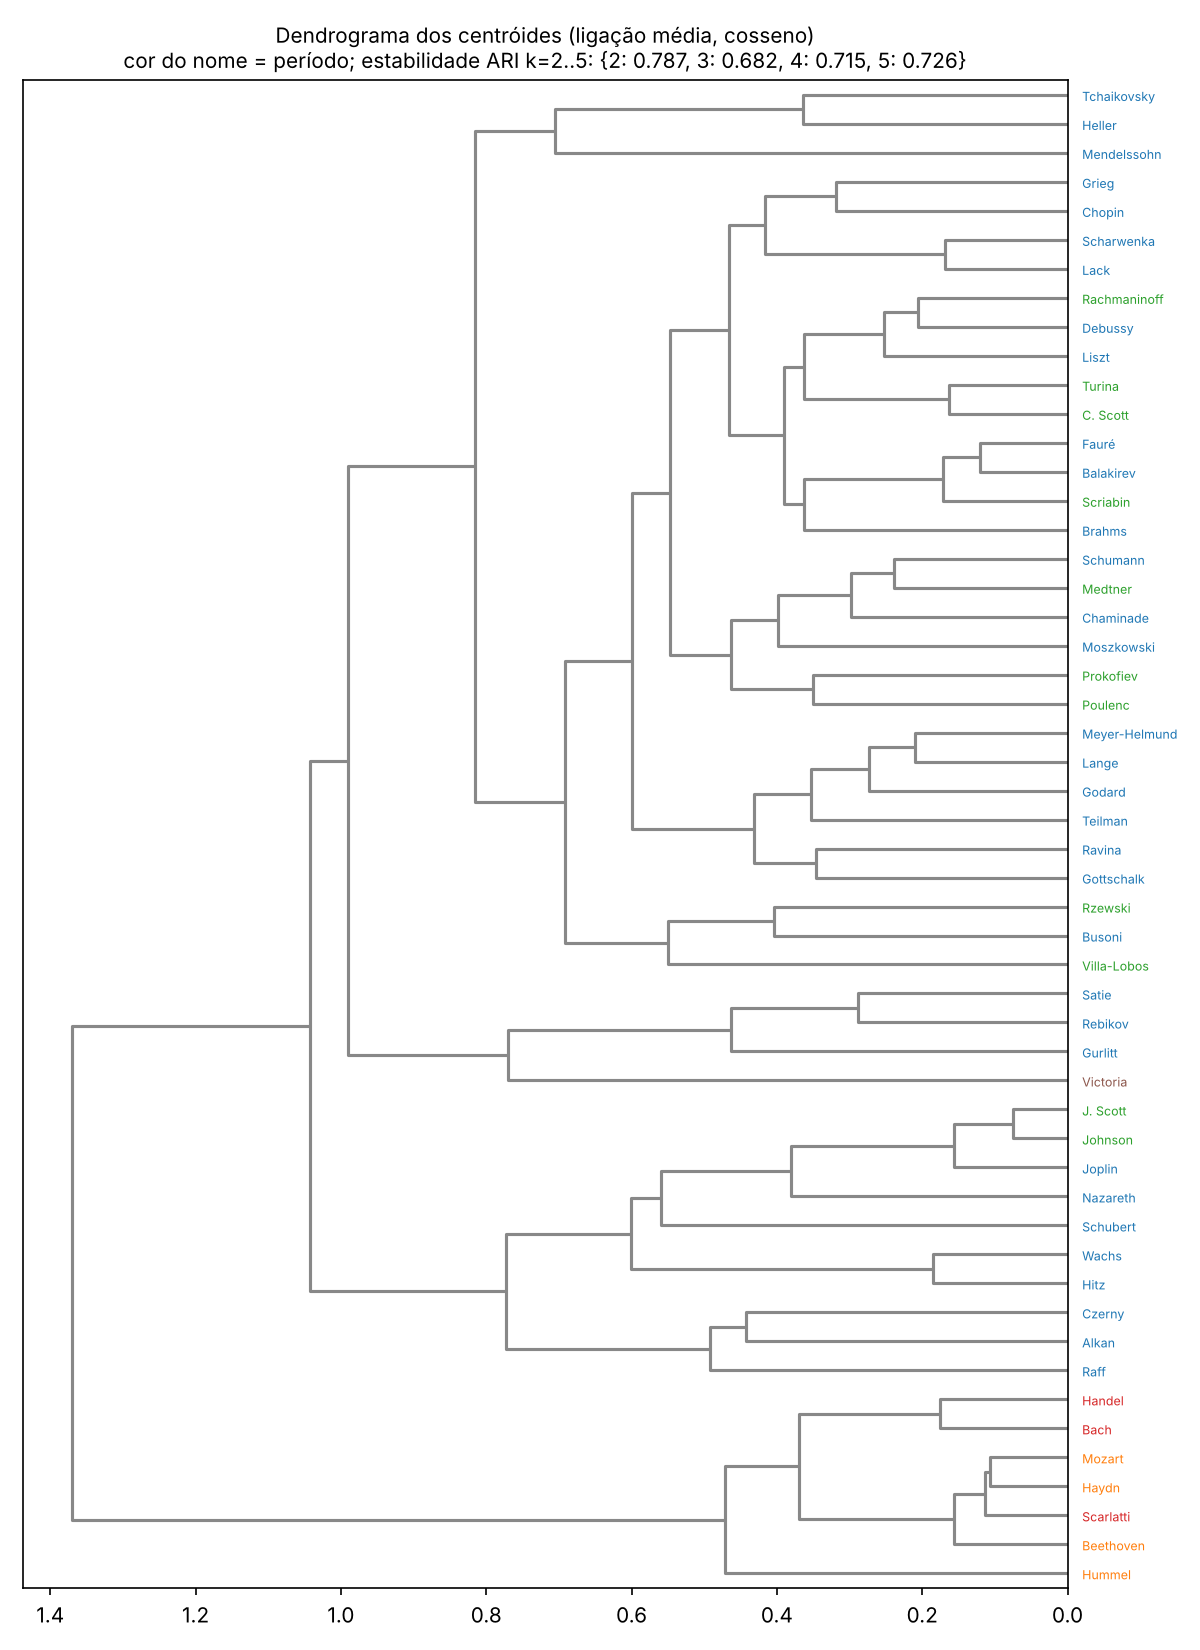
\includegraphics[height=0.78\textheight,width=\linewidth,keepaspectratio]{figuras/dendrograma.png}
    \end{column}
    \begin{column}{0.56\linewidth}
      {\large Bach, Handel, Scarlatti, Haydn, Mozart, Beethoven e Hummel se separam cedo, e o corte se repete em reamostragens (\destaque{ARI 0,79}).\par}
      \vspace{1.5em}
      {\large Os outros 45 se juntam sem fronteira nítida: nenhuma lacuna é maior que a de uma nuvem sem grupos.\par}
    \end{column}
  \end{columns}
  \note{[Thiago] Perguntamos se os compositores formam ilhas ou uma paisagem contínua. Na árvore, compositores parecidos se juntam primeiro, embaixo; quanto mais alto se unem, mais diferentes são. A resposta é quase só paisagem: não há lacuna maior do que a de uma nuvem sem grupos (razão 1,91 contra 2,38 do nulo). A exceção é um bloco de sete compositores, de Bach a Beethoven, que se separa do resto e continua separado quando refazemos a conta com as peças sorteadas de novo. Os 45 demais vão se juntando sem fronteira nítida.

  Cuidado: chamar de “pré-romântico”, não “Barroco” (inclui clássicos); há só 3 barrocos e 4 clássicos. Com 52 pontos o teste tem pouca potência: não concluir que “não existem grupos”. Com 3 trechos por peça o bloco ganha Mendelssohn e Victoria.}
\end{frame}

% =====================================================================
% 9. Steering
% =====================================================================
\begin{frame}{O vetor de Chopin empurra Bach na direção de Chopin}
  \figura{0.65}{figuras/steering.png}
  \vfill
  \legenda{Numa régua de 0 (Bach) a 1 (Chopin), a continuação chega a \destaque{0,68} com o vetor de Chopin, contra 0,43 com um vetor aleatório e 0,39 sem vetor (7 de 7 sementes). Avança, mas não vira Chopin.}
  \vspace{0.3em}
  \note{[Thiago] Aqui invertemos o caminho: em vez de só olhar, mexemos. Pedimos ao modelo que continue um trecho de Bach somando o vetor de Chopin (centro de Chopin menos o centro geral) ao seu estado interno na camada 6, enquanto ele gera. Depois lemos a continuação de novo, sem vetor, e medimos onde ela cai numa régua em que 0 é o centro de Bach e 1 é o centro de Chopin: sem vetor, 0,39; com um vetor aleatório do mesmo tamanho, 0,43; com o de Chopin, 0,68. Quanto mais forte o vetor, mais a música avança (de 0,38 a 0,75). Mas não vira Chopin: anda uns dois terços da régua. Medido sem o modelo, o vetor deixa as notas mais longas e menos densas; o cromatismo não muda (reserva).

  Cuidado: 7 sementes (p = 0,016 é o menor possível), sem escuta sistemática. O eixo de medida é o mesmo que o vetor empurra. Funciona em 3 de 4 pares (falha em Joplin → Chopin; Haydn → Mozart não é interpretável). Steering rodado na base com cópias. Ao gerar músicas para escuta, muitas continuações com vetor degeneraram (tempo voltando para trás): ponto aberto.}
\end{frame}

% =====================================================================
% 10. Surpresa
% =====================================================================
\begin{frame}{A surpresa do modelo cresce com a época}
  \begin{columns}[c,totalwidth=\linewidth]
    \begin{column}{0.4\linewidth}
      \centering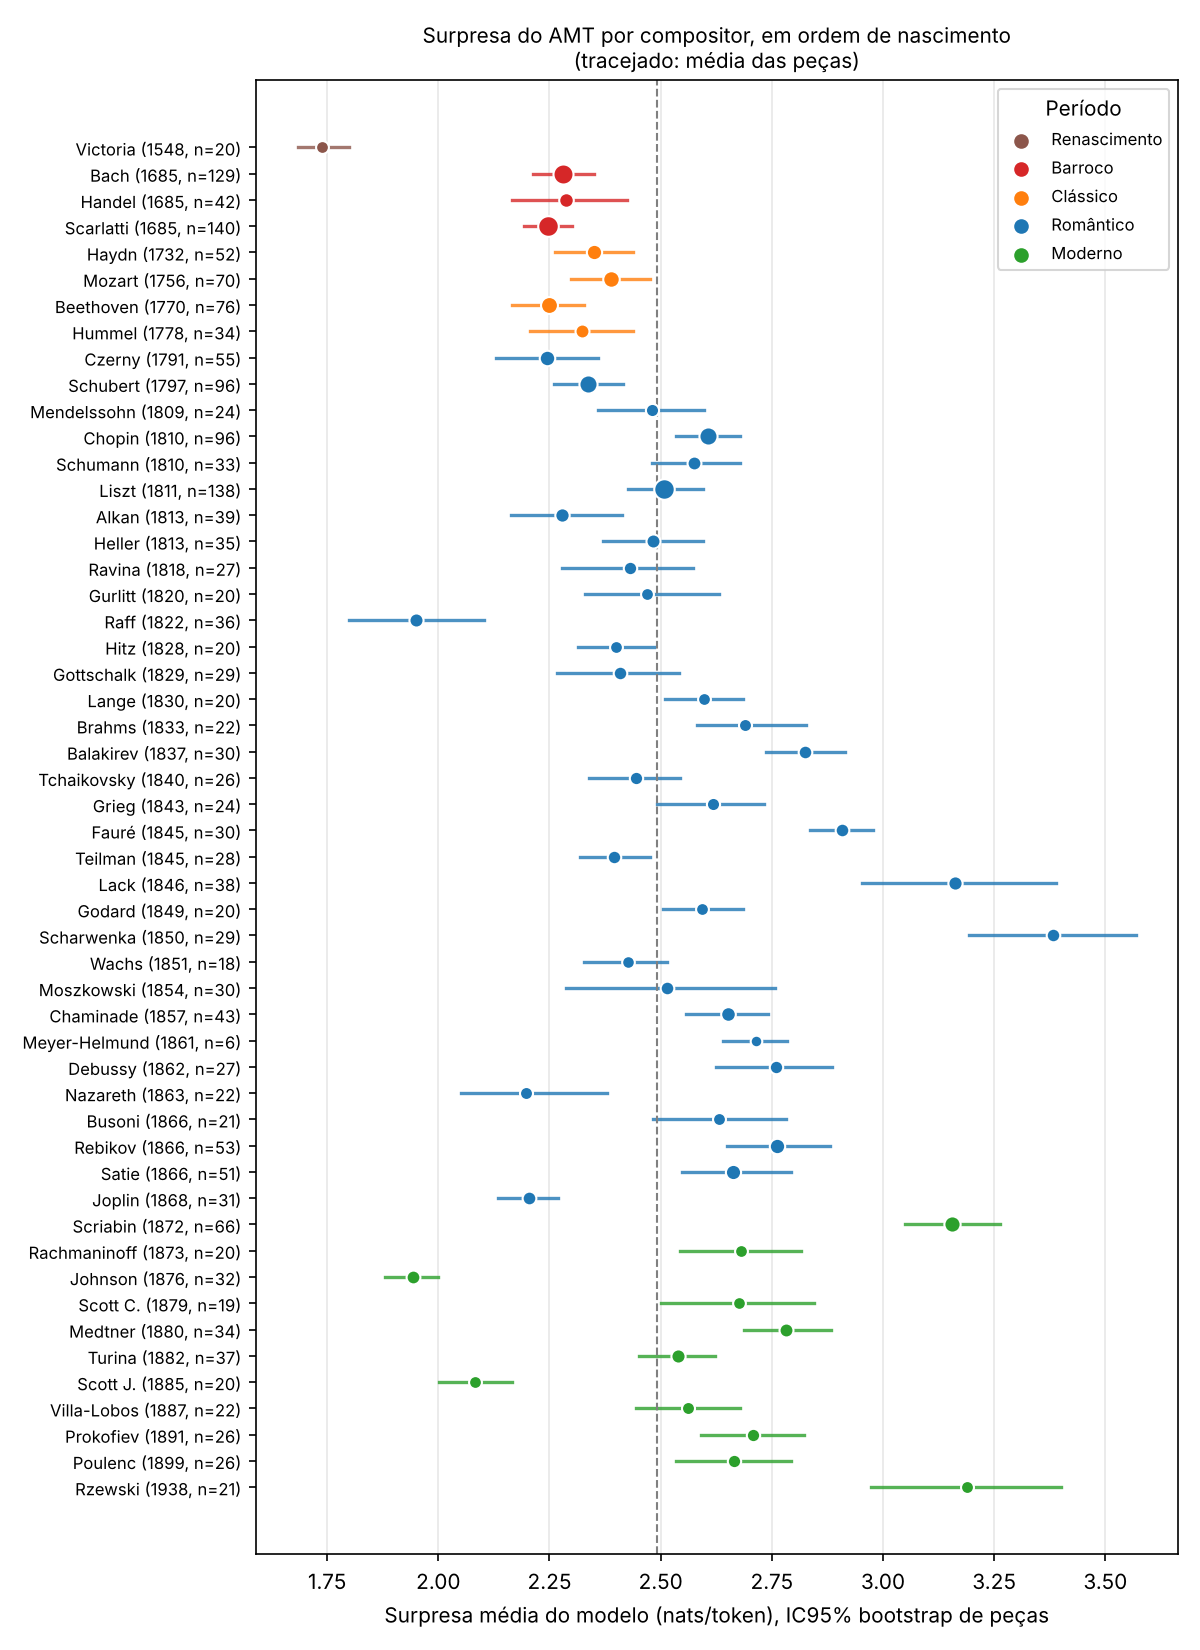
\includegraphics[height=0.78\textheight,width=\linewidth,keepaspectratio]{figuras/surpresa.png}
    \end{column}
    \begin{column}{0.56\linewidth}
      {\large Quanto mais recente o compositor, mais o modelo erra ao prever a próxima nota: correlação de \destaque{0,50} com o ano de nascimento.\par}
      \vspace{1.2em}
      {\normalsize
      \begin{tabular}{@{}llll@{}}
        {\color{cinza}Barroco} & {\color{cinza}Clássico} & {\color{cinza}Romântico} & {\color{cinza}Moderno}\\
        \midrule
        2,27 & 2,32 & 2,54 & 2,69\\
      \end{tabular}\par}
      \vspace{1.2em}
      {\large Descontando densidade, polifonia e duração, ainda 0,40. É a surpresa deste modelo, não a de um ouvinte.\par}
    \end{column}
  \end{columns}
  \note{[Tomaz] Na ideia de Meyer, expectativa importa para o estilo. Medimos o quanto o modelo se surpreende com cada compositor: a perda média por token, ou seja, o quanto ele erra ao prever o próximo token. Na figura, os compositores estão em ordem de nascimento, de cima para baixo; quanto mais à direita, mais surpresa. Victoria é o mais previsível e Scharwenka o mais surpreendente. Em média, quanto mais recente, maior a surpresa. Controlando densidade, polifonia e duração, a correlação cai de 0,50 para 0,40 (p = 0,003), mas não some.

  Cuidado: perda baixa não é “música simples” nem a expectativa de Meyer: é previsibilidade para um modelo treinado no Lakh. Pode refletir quanto cada repertório aparece no Lakh, ruído de transcrição e tamanho do acervo (Barroco com 3 compositores, Clássico com 4). IC95\% da correlação: 0,24 a 0,74.}
\end{frame}

% =====================================================================
% 11. À luz de Meyer
% =====================================================================
\begin{frame}{À luz de Meyer: níveis que existem, mas graduais e frouxos}
  \vfill
  {\normalsize
  \renewcommand{\arraystretch}{1.35}
  \begin{tabular}{@{}>{\raggedright\arraybackslash\bfseries}p{0.22\linewidth}>{\raggedright\arraybackslash}p{0.52\linewidth}>{\raggedright\arraybackslash\bfseries\color{azul}}p{0.2\linewidth}@{}}
    {\mdseries\color{cinza}Nível} & {\color{cinza}O que aparece no modelo} & {\mdseries\color{cinza}Número}\\
    \midrule
    Época (dialeto) & Distância cresce com a diferença de época; só o bloco pré-romântico se separa & correlação 0,50\\
    Compositor (idioma) & Reconhecível, mas uma nuvem que se sobrepõe às vizinhas & 27\% da variação\\
    Obra (escolhas) & Trechos da mesma peça mais próximos entre si (mistura gravação e arquivo) & 52 de 52 compositores\\
    Restrições e escolhas & O vetor médio empurra a música, mas ela não vira o alvo & 0,68 da régua\\
    \bottomrule
  \end{tabular}\par}
  \vfill
  \note{[Tomaz] Lendo à luz de Meyer, o modelo parece ter um nível de dialeto de época, que muda de forma gradual, e um idioma de compositor reconhecível mas frouxo. Dentro de cada obra há coerência, em parte: os dois trechos de uma mesma peça se parecem mais entre si do que com outras peças do autor (diferença 0,33; IC95\% 0,30 a 0,36), mas isso se mistura com a gravação e o arquivo MIDI, que são os mesmos nos dois trechos. E o vetor médio de um compositor captura parte das restrições de um estilo, mas a música ainda faz escolhas que ele não fixa. É uma leitura interpretativa, não uma prova de que o modelo “entende” estilo.

  Ideia opcional: o estilo aparecer gradual e frouxo pode não ser defeito do modelo, e sim uma descrição razoável de como estilos se comportam: categorias que usamos com nitidez são, nos dados, zonas de um contínuo.}
\end{frame}

% =====================================================================
% 12. Síntese
% =====================================================================
\begin{frame}{O que a análise sustenta, e o que não}
  \vspace{0.8em}
  \bloco{0.3\linewidth}{Sustenta}{%
    Distância acompanha a época (0,50), mesmo sem superfície (0,36)\par\vspace{0.6em}
    O compositor explica uma minoria da variação (27\%)\par\vspace{0.6em}
    Um contínuo com um bloco pré-romântico\par\vspace{0.6em}
    O vetor desloca a música em 3 de 4 pares}\hfill
  \bloco[ocre]{0.3\linewidth}{Não se confirmou}{%
    Nacionalidade aproximar compositores\par\vspace{0.6em}
    Finais de obra mais convencionais\par\vspace{0.6em}
    Obras tardias “mais à frente” no mapa}\hfill
  \bloco[tijolo]{0.3\linewidth}{Não dizemos}{%
    Que o mapa é uma linha do tempo\par\vspace{0.6em}
    Que a música virou Chopin\par\vspace{0.6em}
    Que o modelo entende estilo como um ouvinte}
  \note{[Tomaz] Em resumo, três coisas se sustentam: a distância no modelo acompanha a época, de forma moderada e mesmo sem a superfície; o compositor explica uma minoria, então estilo é mais nuvem do que ponto; e o espaço é contínuo, com um bloco de Bach a Beethoven. O vetor do compositor desloca a música em 3 de 4 pares, todos entre compositores distantes. E algumas hipóteses não se confirmaram: nacionalidade não aproxima compositores (rho parcial 0,04), finais de obra não são mais convencionais (diferença de 1\%), e as obras tardias de um compositor não ficam “mais à frente” no mapa (só Chopin mostra o efeito). Preferimos dizer isso com clareza a vender um resultado mais bonito.

  Cuidado: os controles são lineares e simples. p = 0,016 com 7 sementes é o menor possível, não “muito forte”.}
\end{frame}

% =====================================================================
% 13. Próximos passos
% =====================================================================
{\setbeamercolor{background canvas}{bg=tinta}
 \setbeamercolor{normal text}{fg=fundo}
 \setbeamercolor{frametitle}{fg=fundo}
 \setbeamercolor{page number in head/foot}{fg=cinzaescuro}
\begin{frame}{Próximos passos}
  \usebeamercolor[fg]{normal text}
  \vspace{0.6em}
  \bloco[azulclaro]{0.22\linewidth}{Ouvir}{\color{claroescuro}Escuta sistemática das continuações: o teste mais direto de estilo}\hfill
  \bloco[azulclaro]{0.22\linewidth}{Mais pares}{\color{claroescuro}Só 4 pares e 7 sementes por par foram testados}\hfill
  \bloco[azulclaro]{0.22\linewidth}{Controles}{\color{claroescuro}Andamento, dinâmica e superfície de forma não linear}\hfill
  \bloco[azulclaro]{0.22\linewidth}{Outro modelo}{\color{claroescuro}Repetir com um modelo treinado em música clássica}
  \vfill
  {\fontsize{18}{22}\selectfont\bfseries O que, no estilo, é invisível para uma máquina que só vê notas e tempos?\par}
  \vspace{1em}
  {\color{claroescuro}Para explorar (páginas na pasta \texttt{html/}):
   \href{run:html/explorador.html}{mapa interativo dos 52 compositores} ·
   \href{run:html/escuta/index.html}{trechos gerados para ouvir}\par}
  \vspace{0.3em}
  \note{[Tomaz] Falta uma escuta sistemática das continuações geradas, que seria o teste mais direto de estilo. Falta testar mais pares de compositores, controlar andamento, dinâmica e superfície de forma não linear, e repetir com um modelo treinado em música clássica. Quem quiser pode explorar o mapa e ouvir os trechos gerados: as duas páginas estão na pasta html/ e abrem em qualquer navegador. Para quem faz arte, a pergunta continua aberta: o que, no estilo, é invisível para uma máquina que só vê notas e tempos?

  Cuidado: nada disso foi feito; apresentar como proposta. Terminar na pergunta.}
\end{frame}
}

% =====================================================================
% Agradecimento (sem número)
% =====================================================================
{\setbeamercolor{background canvas}{bg=tinta}
\begin{frame}[plain,noframenumbering]
  \vspace*{0.4cm}
  {\color{cinzaescuro}\large Artes e Ciência · IMPA Tech · novembro de 2026\par}
  \vfill
  {\color{fundo}\fontsize{44}{48}\selectfont\bfseries Obrigado!\par}
  \vspace{0.6em}
  {\color{claroescuro}\large Perguntas são bem-vindas.\par}
  \vfill
  {\color{fundo}\large Lucas Barbosa · Thiago Vinicius · Tomaz L. Cavalcante\par}
  \vspace{0.3em}
  {\color{cinzaescuro}Mapa interativo e trechos para ouvir: links no slide anterior\par}
  \vspace*{0.3cm}
  \note{Agradecer e abrir para perguntas. Os slides de reserva vêm depois deste: só usar se alguém perguntar sobre camadas, compositores à frente do tempo, outros pares, o que o vetor muda ou o eixo do tempo.}
\end{frame}
}

% =====================================================================
% Reserva
% =====================================================================
{\setbeamercolor{background canvas}{bg=tinta}
\begin{frame}[plain]
  \vfill
  {\color{fundo}\fontsize{34}{38}\selectfont\bfseries Reserva\par}
  \vspace{0.8em}
  {\color{claroescuro}\large Camadas do modelo · à frente ou atrás do tempo · outros pares · o que o vetor muda · o que o eixo do tempo acompanha\par}
  \vfill
  \note{Não apresentar. Usar só se perguntarem. Finais de obra (não se confirmou): diferença de cerca de 1\% da distância ao centro do período; 52,8\% das peças na direção esperada; sinal oposto no Barroco e no Clássico.}
\end{frame}
}

\begin{frame}{As camadas do meio separam melhor os compositores}
  \figura{0.65}{figuras/camadas.png}
  \vfill
  \legenda{Os vetores vêm da \destaque{camada 6 de 12}: acerto de 0,31, contra 0,19 na última (acaso: 0,019). As camadas 5 a 9 são parecidas.}
  \vspace{0.3em}
  \note{Se perguntarem por que a camada 6. Escolhemos a camada numa grade de camadas e formas de média, pelo acerto do classificador somado à estabilidade. Sem as cópias, a camada 7 empatou com a 6 pelo critério; mantivemos a 6, decisão registrada no diário. O mesmo estado da camada 6 é usado no mapa, nas nuvens e no steering (o vetor é somado na saída do 6.º bloco). Cada número é uma execução, sem intervalo; camada escolhida e avaliada nos mesmos dados. Não dizer que o modelo “sabe menos” na última camada: ela é especializada em prever o próximo token.}
\end{frame}

\begin{frame}{À frente ou atrás do tempo (só ilustração)}
  \figura{0.65}{figuras/tempo.png}
  \vfill
  \legenda{\destaque{36 de 52} compositores ficam fora da reta entre época e posição no mapa. Os clássicos soam “mais antigos” que a data; o romantismo médio e tardio, “mais moderno”.}
  \vspace{0.3em}
  \note{Cuidado: posição no mapa, não juízo de inovação. O intervalo mede só a amostragem das peças, sem a incerteza da reta (R² 0,32) nem da projeção; desvios de grupo geram desvios “significativos” em bloco; Victoria tem muita influência na reta. As obras tardias de um compositor não ficam mais “à frente” (não se confirmou; só Chopin mostra o efeito).}
\end{frame}

\begin{frame}{O vetor não funciona em todo par de compositores}
  \figura{0.65}{figuras/steering_pares.png}
  \vfill
  \legenda{Desloca em \destaque{3 de 4} direções interpretáveis: Bach → Chopin, Chopin → Bach e Mozart → Debussy. Falha em Joplin → Chopin; Haydn → Mozart estão sobrepostos demais para medir.}
  \vspace{0.3em}
  \note{Dizer: “funciona entre estilos distantes; não é garantido para qualquer par”. Joplin → Chopin: 5 de 7 sementes, p = 0,69. Steering rodado na base com cópias.}
\end{frame}

\begin{frame}{O que o vetor muda na música, medido sem o modelo}
  \figura{0.65}{figuras/descritores.png}
  \vfill
  \legenda{Com o vetor de Chopin, Bach cai de 9,0 para \destaque{4,8 notas por segundo} e as notas se alongam. O andamento segue o alvo; a polifonia sobe com qualquer alvo; o cromatismo não se move.}
  \vspace{0.3em}
  \note{Duração das notas: sobe com Chopin (0,30 → 0,65 s) e com Debussy (0,29 → 1,05 s), não com Joplin. Com o vetor de Joplin, a densidade sobe (15,3 → 18,5 notas/s). Polifonia: 2,4 → 3,0; 2,4 → 4,6; 3,6 → 4,2.

  Cuidado: 7 sementes, vários testes sem correção, continuações de 40 notas. Contra “sem vetor”, as mudanças de Joplin não chegam a p < 0,05; a evidência vem do contraste com o vetor aleatório.}
\end{frame}

\begin{frame}{O que o eixo do tempo do mapa acompanha}
  \figura{0.65}{figuras/eixos.png}
  \vfill
  \legenda{Por compositor, o eixo horizontal do mapa acompanha polifonia e duração (\destaque{0,85}) e, menos, o cromatismo (0,60). Ler só o painel da esquerda.}
  \vspace{0.3em}
  \note{Ler a barra dos compositores. O painel do segundo eixo tem sinal arbitrário. Correlação, não mecanismo: gênero, instrumento e gravação se confundem com a época; n = 52. Polifonia e duração provavelmente são redundantes. É coerente com a queda de 0,50 para 0,36 no controle de superfície.}
\end{frame}

\end{document}
